\chapter{Аналитическая часть}

В этом разделе рассматриваются объекты сцены, способы их представления и существующие алгоритмы создания изображений, а также осуществляется выбор наиболее подходящих из этих алгоритмов для дальнейшего применения.

\section{Формализация объектов сцены}

Сцена является набором объектов, включащим в себя:

\begin{enumerate}
	\item объекты сцены -- геометрические многогранные примитивы, расположенные в пространстве сцены, такие как, куб, прямая призма треугольная пирамида. Каждый примитив состоит из граней, сформированных из точек соединенных ребрами. Геометрические характеристики примитивов задаются параметрами такими, как длина ребра основания, высота, радиусы описанных окружностей нижнего и верхнего основания, количество боковых граней. Спектральные характеристики так же задаются параметрами такими, как коэффициенты отражения и блеска, цвет.
	\item источник света -- пространственный вектор, указывающий направление света. Свет всегда направлен вдоль положительной оси $Z$, его положение в пространстве сцены задается пользователем.
	\item камера -- пространственный вектор, указывающий направление просмотра.
\end{enumerate}

\section{Анализ способов представления модели}

\begin{enumerate}
	\item \textit{каркасная модель} -- простейший способ представления моделей, основанный на использовании точек и рёбер, содержащий минимум иформации и имеющий ряд ограничений. Основным недостатком является неоднозначность, так как невозможно четко определить ориентацию и видимость, что может привести к непредсказуемым результатам. Удаление скрытых линий требует ручного редактирования, что может разрушить целостность модели. 
	\begin{figure}[h] 
		\centering
		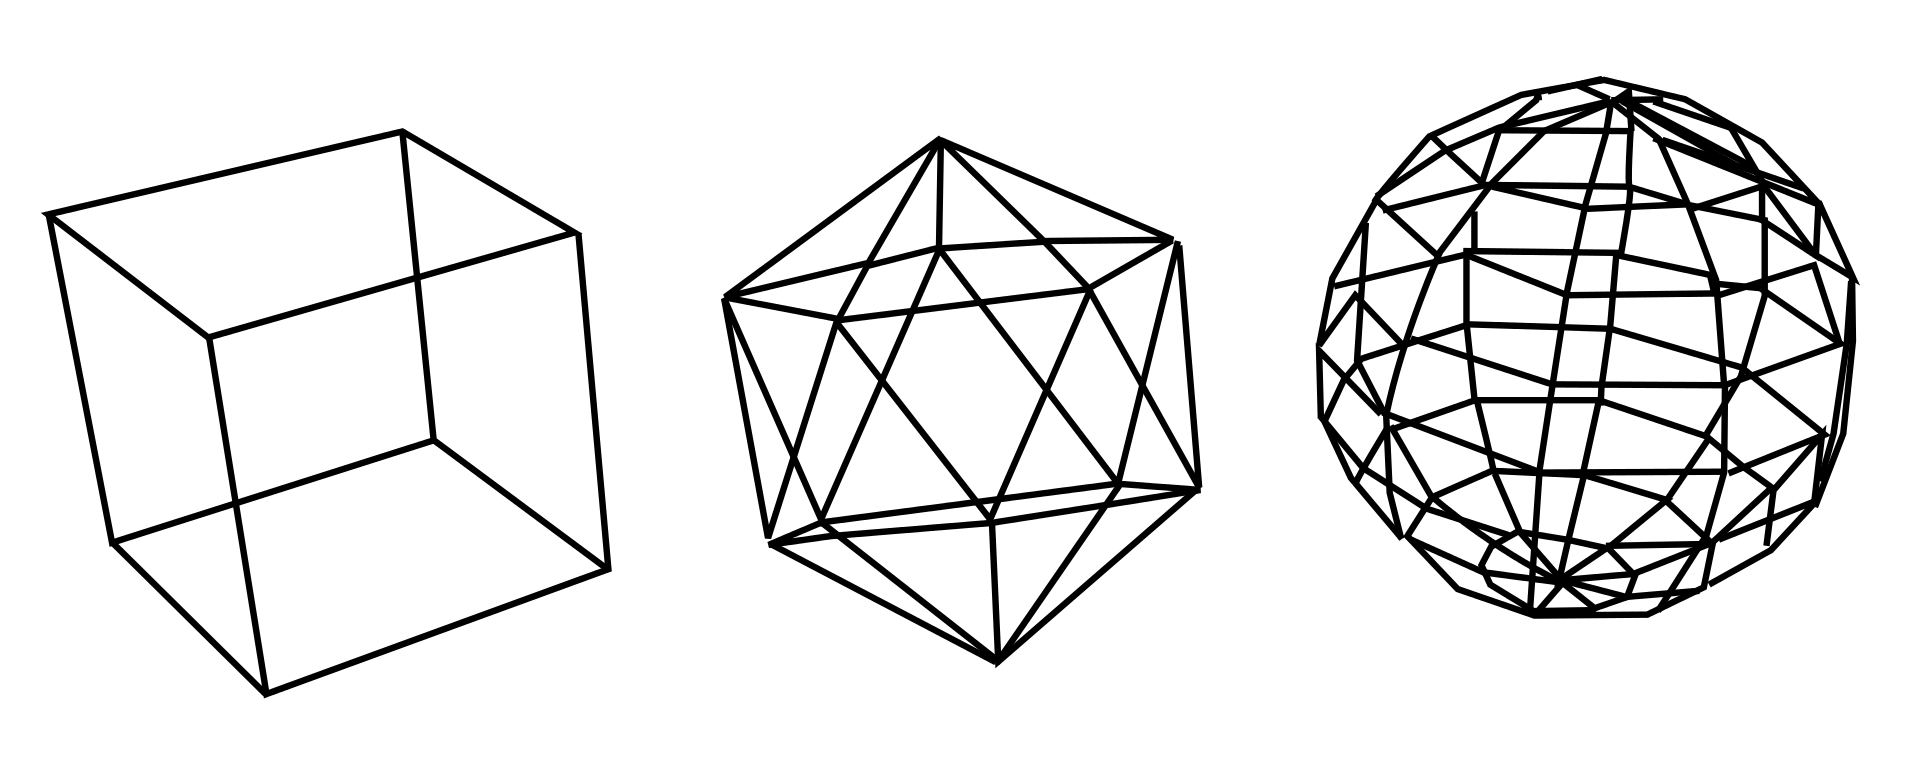
\includegraphics[width=0.6\textwidth]{images/carcass-models.png}
		\caption{Каркасные модели} 
		\label{fig:carcass-models} 
	\end{figure}
	Также каркасные модели не поддерживают технику тонового изображения, так как затенение применяется к граням, а не к ребрам, что ограничивает их использование в задачах, требующих визуальной глубины и реалистичности. Несмотря на эти ограничения, каркасные модели требуют меньше памяти и легки в отрисовке. Пример каркасных моделей приведён на рисунке \ref{fig:carcass-models}.
	
	\item \textit{поверхностная модель} -- способ представления моделей, основанный на использовании точек, линий и поверхностей, что делает его более гибким и многофункциональным по сравнению с каркасной моделью. Он позволяет изображать сложные криволинейные грани, создавать тоновые трехмерные изображения и выявлять особенности, такие как отверстия. Этот метод обеспечивает высокое качество изображений. Поверхностную модель можно задать двумя способами:
	\begin{itemize}[label=--]
		\item \textit{параметрическое представление} -- вид поверхностной модели, требующий вычисления функции, зависящей от параметра, но его использование затруднено в сценах без поверхностей вращения;
		\item \textit{полигональная сетка} -- вид поверхностной модели, представленный совокупностью вершин, рёбер и граней. Гранями обычно являются треугольники, четырёхугольники или другие простые выпуклые многоугольники, но могут также являться многоугольниками с отверстиями. Пример поверхностной модели, заданной полигональной сеткой, приведён на рисунке \ref{fig:polygonal-models}.
	\end{itemize}
	\begin{figure}[h] 
		\centering
		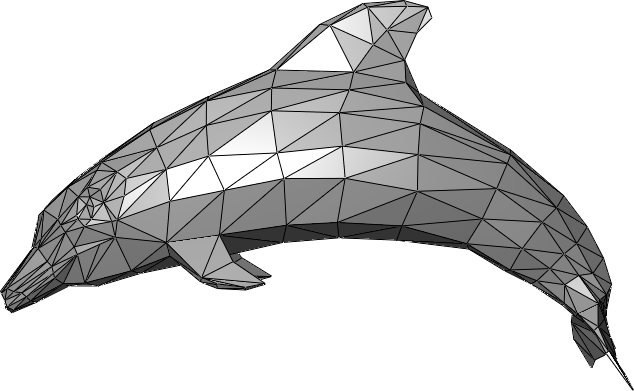
\includegraphics[width=0.5\textwidth]{images/polygonal-models.png}
		\caption{Поверхностая модель, заданная полигональной сеткой} 
		\label{fig:polygonal-models} 
	\end{figure}
	Однако у поверхностной модели есть недостаток: она не предоставляет информации о том, с какой стороны поверхности находится материал.
	
	\item \textit{твердотельная модель} -- способ представления моделей, включающий информацию о внутренней структуре и расположении материала, в отличие от поверхностной модели, что достигается указанием направления внутренней нормали.
	\begin{figure}[h] 
		\centering
		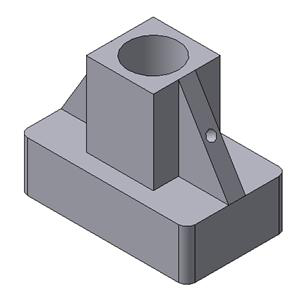
\includegraphics[width=0.5\textwidth]{images/solidum-statu-models.png}
		\caption{Твердотельная модель} 
		\label{fig:solidum-statu-models} 
	\end{figure}
	Твердотельные модели обладают неоспоримыми преимуществами, включая полное определение объемной формы с разграничением внешних и внутренних областей, что позволяет избежать нежелательных взаимовлияний компонентов. Они обеспечивают автоматическое удаление скрытых линий и построение трехмерных разрезов, что важно для анализа сложных композиций. Пример твердотельной модели приведён на рисунке \ref{fig:solidum-statu-models}.
\end{enumerate}
	
Для выполнения данной работы каркасная модель не подходит, так как она может исказить восприятие форм объекта. Твердотельная модель так же не является оптимальной, поскольку в этой работе не требуется информация о материале и его расположении. Таким образом, остается только поверхностная модель как наилучший выбор. Поверхностная модель будет задана полигональной сеткой, так как в этой работе не будет обработки поверхностей вращения и использование параметрического представления избыточно.

\section{Анализ способов представления поверхностной модели, заданной полигональной сеткой}

Объекты, созданные с помощью полигональных сеток, должны хранить разные типы элементов, такие как вершины, рёбра, грани, полигоны и поверхности. Во многих случаях хранятся лишь вершины, рёбра и либо грани, либо полигоны (рис. \ref{fig:polygonal-models-example}). Грани могут быть как трехсторонними, так и четырехсторонними.

\begin{figure}[h] 
	\centering
	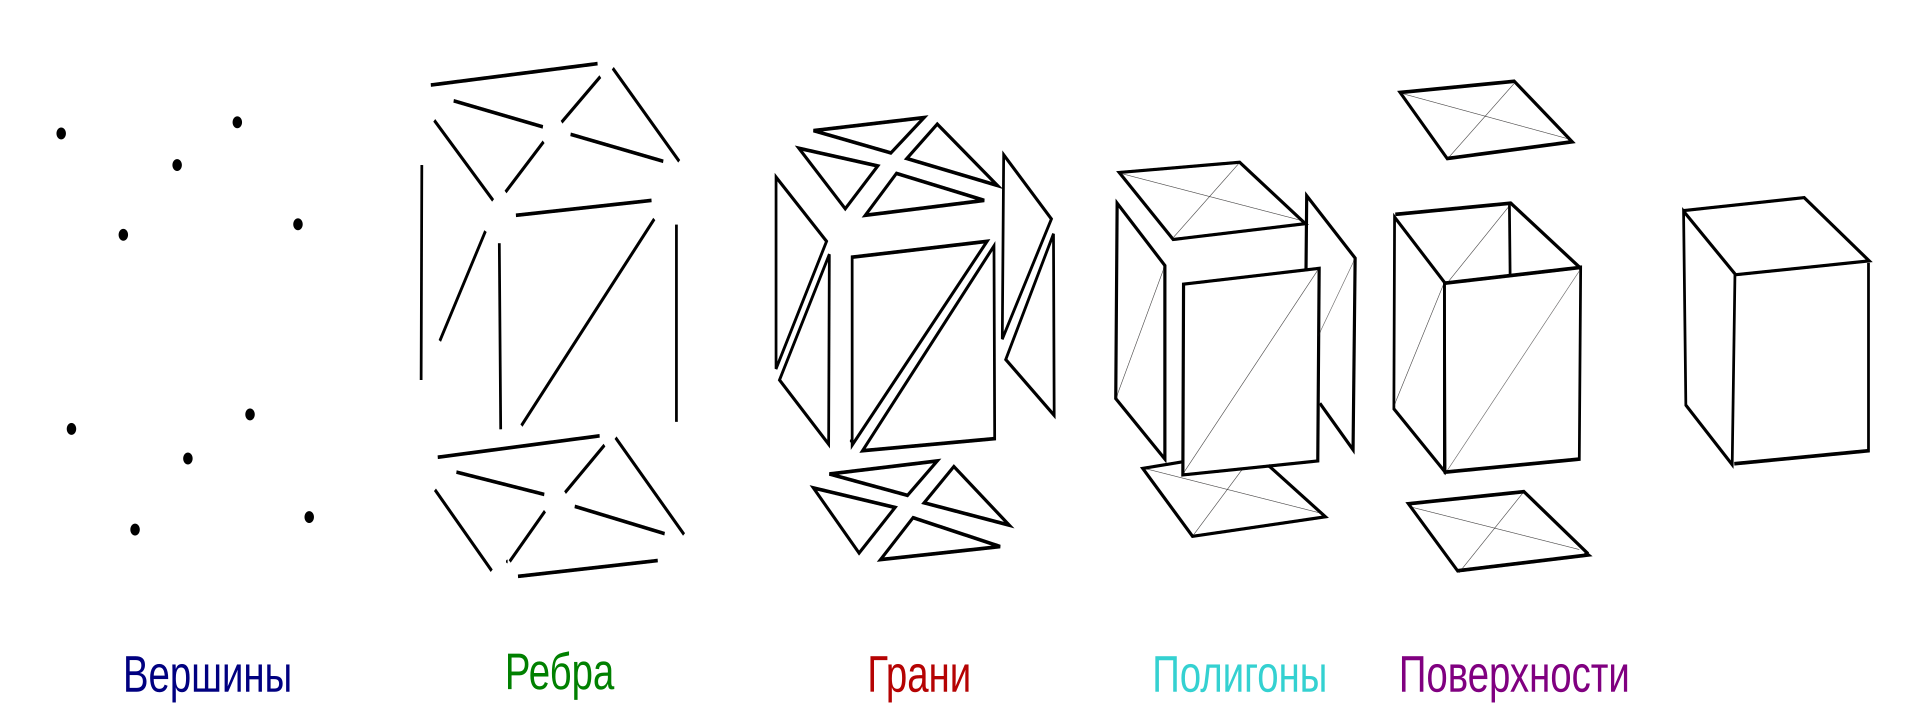
\includegraphics[width=0.7\textwidth]{images/polygonal-models-example.png}
	\caption{Элементы моделирования сетки} 
	\label{fig:polygonal-models-example} 
\end{figure}

\begin{enumerate}
	\item \textit{вершинное представление} -- простейший способ представления, описывающий объект как набор вершин, соединённых с другими вершинами. Хотя это и простейший способ представления, он не так широко используется, поскольку не предоставляет явной информации о гранях и рёбрах. 
	\begin{figure}[h] 
		\centering
		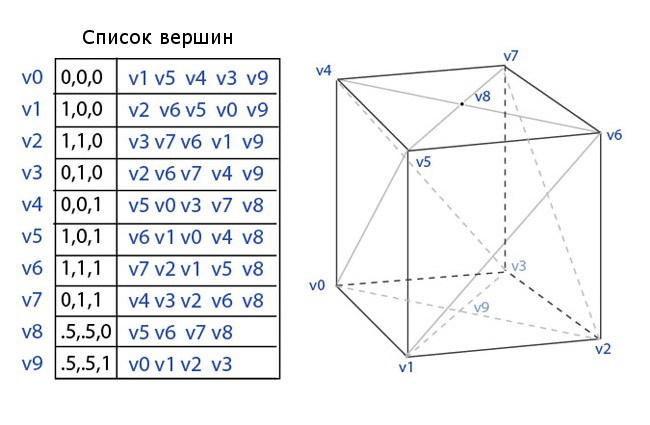
\includegraphics[width=0.7\textwidth]{images/vertex-list.png}
		\caption{Вершинное представление} 
		\label{fig:vertex-list} 
	\end{figure}
	Это означает, что для генерации списка граней, необходимого для рендеринга, нужно обойти все данные, что усложняет выполнение операций с рёбрами и гранями. Пример полигональной сетки, заданной вершинным представлением приведён на рисунке \ref{fig:vertex-list}.
	
	\item \textit{список граней} -- способ представления, описывающий объект как множество вершин и граней, который является наиболее распространённым представлением для современного графического оборудования. Это представление упрощает моделирование, позволяя легко находить грани, окружающие конкретные вершины. Пример полигональной сетки, заданной списком граней приведён на рисунке \ref{fig:planes-list}. 
	\begin{figure}[h] 
		\centering
		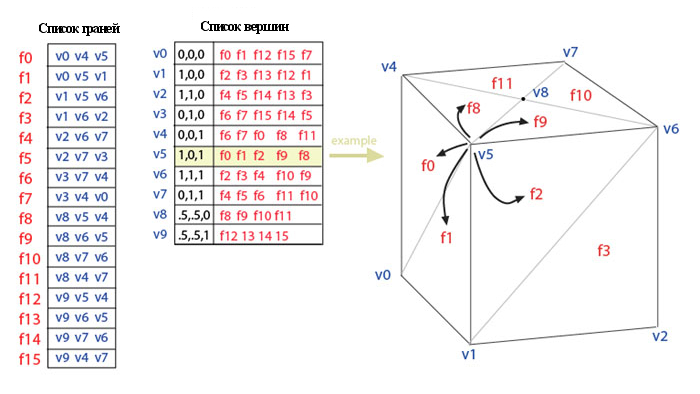
\includegraphics[width=0.8\textwidth]{images/planes-list.png}
		\caption{Список граней} 
		\label{fig:planes-list} 
	\end{figure}
	
	\item \textit{<<крылатое>> представление} -- способ представления, описывающий объект как множество вершин, граней и рёбер, что обеспечивает высокую гибкость в динамическом изменении геометрии. «Крылатое» представление эффективно решает задачу обхода от ребра к ребру, предоставляя упорядоченное множество граней вокруг каждого ребра. Оно включает информацию о двух конечных вершинах, двух гранях и четырёх ближайших рёбрах. Пример полигональной сетки, заданной <<крылатым>> представлением приведён на рисунке \ref{fig:wings-list}. 
	\begin{figure}[h] 
		\centering
		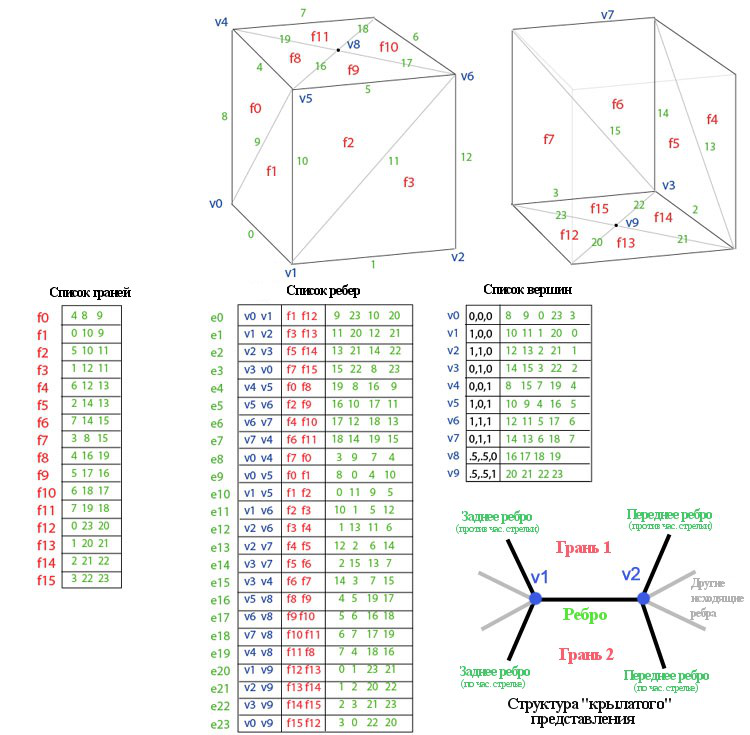
\includegraphics[width=0.8\textwidth]{images/wings-list.png}
		\caption{<<Крылатое>> представление} 
		\label{fig:wings-list} 
	\end{figure}
\end{enumerate}

Для хранения полигональной сетки будет использован метод, основанный на списке граней, что обеспечивает ясное представление о гранях. Этот подход способствует эффективному преобразованию моделей, так как структура включает в себя список вершин.

\section{Анализ алгоритмов удаления невидимых линий и поверхностей}

Главной целью при создании реалистичного изображения является удаление объектов или их частей, которые не видны наблюдателю из-за перекрытия другими объектами. Для решения этой задачи выделяют две категории алгоритмов:

\begin{itemize}[label=--]
	\item \textit{Алгоритмы, работающие в объектном пространстве,} привязаны к мировой или физической системе координат. Их результаты зависят только от точности вычислений и требуют значительных вычислительных ресурсов, что зависит от необходимой точности и сложности входной сцены. К этой категории относятся алгоритмы Робертса, алгоритмы со списком приоритетов и другие.
	
	\item \textit{Алгоритмы, работающие в пространстве изображения,} ориентированы на систему координат экрана или картинной плоскости, на которую проецируются объекты. Объем вычислений в этой группе значительно меньше по сравнению с первой, и он зависит от разрешающей способности экрана и количества объектов в сцене. К основным алгоритмам этой группы относятся алгоритм Варнока, алгоритм Z-буфера и алгоритм трассировки лучей.
\end{itemize}

\subsection{Алгоритм Робертса}

Алгоритм Робертса — это первое известное решение задачи об удалении невидимых линий в трехмерной графике. Он представляет собой математически элегантный метод, работающий в объектном пространстве. Основная задача алгоритма заключается в удалении ребер и граней, которые экранируются самим объектом, а затем в сравнении оставшихся видимых ребер с другими объектами для определения их видимости.

Работа Алгоритма Робертса проходит в два этапа:
\begin{itemize}[label=--]
	\item определение нелицевых граней для каждого тела отдельно;
	\item определение и удаление невидимых ребер.
\end{itemize}

Для корректной работы данного алгоритма, необходимо выполнение следующих предварительных условий:
\begin{itemize}[label=--]
	\item тело ограничено плоскостями;
	\item нормали всех граней направлены внутрь тела;
	\item тело выпукло (невыпуклые тела должны быть разбиты на выпуклые части).
\end{itemize}

В этом алгоритме выпуклое многогранное тело с плоскими гранями должно представиться набором пересекающихся плоскостей. Уравнение произвольной плоскости в трехмерном пространстве имеет вид:
\begin{equation}
	ax + by + cz + d = 0
	\label{eq:plane-eq}
\end{equation}

В матричной форме уравнение \ref{eq:plane-eq} выглядит так:
\begin{equation}
	\begin{pmatrix}
		x & y & z & 1
	\end{pmatrix}
	\begin{pmatrix}
		a \\
		b \\
		c \\
		d \\
	\end{pmatrix}
	= 0
	\label{eq:matrix-plane-eq1}
\end{equation}

Тогда набор пересекающихся плоскостей состоит из матрицы коэффициентов уравнений плоскостей и называется \textit{матрицей тела}:
\begin{equation}
	V = 
	\begin{pmatrix}
		a_1 & a_2 & \cdots & a_n \\
		b_1 & b_2 & \cdots & b_n \\
		c_1 & c_2 & \cdots & c_n \\
		d_1 & d_2 & \cdots & d_n
	\end{pmatrix}
	\label{eq:model-matrix}
\end{equation}

Корректное формирование матрицы тела предполагает, что любая точка внутри него должна находиться по положительную сторону от каждой грани. Если это условие не соблюдено для определенной грани, следует умножить соответствующий столбец матрицы на -1. Для проверки правильности можно взять точку, находящуюся внутри тела, координаты которой вычисляются как среднее значение координат всех его вершин.

Далее удаляются грани, которые скрыты телом. Для этого используется вектор взгляда $E = \begin{pmatrix} 0 & 0 & -1 & 0 \end{pmatrix}$, и чтобы определить невидимые грани, вектор умножается на матрицу тела $V$. Отрицательные компоненты результата указывают на невидимые грани.

Для выявления невидимых точек на ребре необходимо провести луч от наблюдателя к точке наблюдения. Если луч сталкивается с каким-либо объектом, то точка считается невидимой. Если объект действительно препятствует прохождению луча, он должен пересекать этот объект, оставаясь по положительную сторону от каждой его грани.

Вычислительная сложность алгоритма возрастает теоретически как квадрат числа объектов, то есть его главный недостаток -- скорость работы. К тому же, этот алгоритм сложнореализуемый из-за его полностью математической структуры.

Основное преимущество данного алгоритма заключается в высокой точности вычислений, которая достигается благодаря работе в объектном пространстве, в отличие от большинства других алгоритмов.

\subsection{Алгоритм Варнока}

Алгоритм Варнока основывается на гипотезе о том, как человеческий глаз и мозг обрабатывают информацию в сцене. Эта гипотеза утверждает, что на обработку областей с низким информационным содержанием уходит значительно меньше времени и усилий, чем на области с высоким содержанием информации.

Конкретная реализация алгоритма зависит от метода разбиения окна и от критериев, используемых для определения простоты содержимого окна. В оригинальной версии алгоритма каждое окно делится на четыре равных подокна. Многоугольник в изображаемой сцене может быть классифицирован следующим образом (рис. \ref{fig:varnok-models}):
\begin{itemize}[label=--]
	\item \textit{внешний}, если он находится полностью вне окна;
	\item \textit{внутренний}, если он находится полностью внутри окна;
	\item \textit{пересекающий}, если он пересекает границу окна;
	\item \textit{охватывающий}, если окно находится полностью внутри него.
\end{itemize}

\begin{figure}[h] 
	\centering
	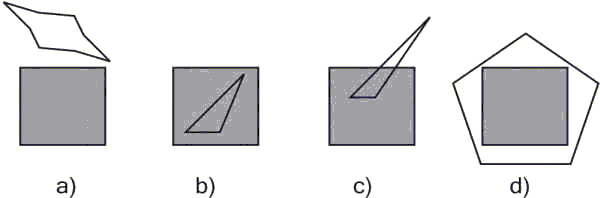
\includegraphics[width=0.8\textwidth]{images/varnok-models.png}
	\caption{Типы многоугольников: внешний (a), внутренний (b), пересекающий (c), охватывающий (d)} 
	\label{fig:varnok-models} 
\end{figure}

Алгоритм можно описать в общих чертах следующим образом:
\begin{enumerate}
	\item если все многоугольники сцены являются внешними по отношению к окну, то окно считается пустым, заполняется фоновым цветом и дальнейшему разбиению не подлежит.
	\item если только один многоугольник пересекает окно и является внутренним, окно заполняется фоновым цветом, а сам многоугольник — своим цветом.
	\item если только один многоугольник пересекает окно и является пересекающим, окно заполняется фоновым цветом, а часть многоугольника, которая принадлежит окну, заполняется цветом этого многоугольника.
	\item если только один многоугольник охватывает окно и нет других многоугольников, имеющих общие точки с окном, то окно заполняется цветом этого многоугольника.
	\item если существует хотя бы один охватывающий окно многоугольник, из всех таких выбирается тот, который ближе всего к точке наблюдения, и окно заполняется его цветом.
	\item в противном случае производится новое разбиение окна.
\end{enumerate}

\begin{figure}[h] 
	\centering
	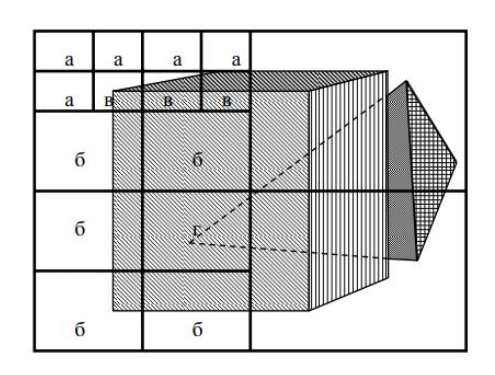
\includegraphics[width=0.6\textwidth]{images/varnok.png}
	\caption{Пример разбиения алгоритмом Варнока} 
	\label{fig:varnok} 
\end{figure}

Шаги 1–4 рассматривают случай пересечения окна только с одним многоугольником, что помогает уменьшить количество подразбиений. Шаг 5 решает проблему удаления невидимых поверхностей, так как многоугольник, находящийся ближе к наблюдателю, экранирует остальные. Пример разбиения приведён на рисунке \ref{fig:varnok}.

Основной недостаток алгоритма заключается в его рекурсивной работе. На каждом этапе он проверяет, какие грани видны, и если определение видимости нетривиально, окно разделяется на четыре секции, и анализ проводится отдельно для каждой из них.

\section*{Вывод}

<что сделали в аналите, кратко>

\begin{itemize}
	\item test
\end{itemize}

\clearpage
